%%%%%%%%%%%%%%%%%%%%%%%%%%%%%%%%%%%%%%%%%%%%%%%%%%%%%%%%%%%%%%%%%%%%%%%%%%%%%%%
%%% SETUP

\providecommand{\main}{../..}  % for subfiles
\providecommand{\mystyleloc}{../../util}  % for stylesheets
\documentclass[\main/main.tex]{subfiles}

%%%%%%%%%%%%%%%%%%%%%%%%%%%%%%%%%%%%%%%%%%%%%%%%%%%%%%%%%%%%%%%%%%%%%%%%%%%%%%%
%                                 SETTINGS
%%%%%%%%%%%%%%%%%%%%%%%%%%%%%%%%%%%%%%%%%%%%%%%%%%%%%%%%%%%%%%%%%%%%%%%%%%%%%%%
% Implementing Package Settings

\graphicspath{{images/}{\main/images/}}

\title{General Qualifying Exam Solutions: Galaxies\\}
\author{{Starkman}, Nathaniel \\%
		\and {Lokken}, Martine \\%
		\and {Ludwig}, Bethany \\%
		\and {Sheere}, Connor \\%
		\and {Winch}, Harrison%
}
% \date{\today}


%%%%%%%%%%%%%%%%%%%%%%%%%%%%%%%%%%%%%%%%%%%%%%%%%%%%%%%%%%%%%%%%%%%%%%%%%%%%%%%
%                                  DOCUMENT
%%%%%%%%%%%%%%%%%%%%%%%%%%%%%%%%%%%%%%%%%%%%%%%%%%%%%%%%%%%%%%%%%%%%%%%%%%%%%%%

\begin{document}

% -----------------------------------------------------------------------------
%                                  TITLE PAGE
% -----------------------------------------------------------------------------

\maketitle

% -----------------------------------------------------------------------------
%                                     TOC
% -----------------------------------------------------------------------------

\tableofcontents
\let\tableofcontents\relax


% -----------------------------------------------------------------------------
%                                    INTRO
% -----------------------------------------------------------------------------

\newpage
\section{Introduction} % (fold)
\label{sec:introduction}


	% External Answers

% section introduction (end)

\newpage


% -----------------------------------------------------------------------------
%                                      Q1
% -----------------------------------------------------------------------------

\section{Q1) Mass of the Milky Way} % (fold)
\label{sec:q1_mass_of_the_milky_way}
\questiontext{What is the total mass (in both dark matter and in stars) of the Milky Way galaxy? How does this compare to M31 and to the LMC? How is this mass determined?}


	\subsubsection{Short Answer} % (fold)
	\label{ssub:q1_short_answer}

		\begin{table}[H]
			\centering
			\caption{Galaxy Masses}
			\label{tab:my-table}
			\begin{tabular}{@{}l|ll@{}}
				\toprule
				Object          & Total {[}$M_\odot${]} & Stars {[}$M_\odot${]} \\ \midrule
				Milky Way       & $\approx 1 \times 10^{12}$     & $\lesssim 10^{11}$     \\
				Andromeda (M31) & \multicolumn{2}{c}{$\approx 2 \times M_{MW}$} \\
				LMC             & $\approx 10^{10} $    & $\approx 10^{9}$     \\ \bottomrule
			\end{tabular}
		\end{table}


		There are variety of methods to determine the total masses of these objects. For more details, besides the included notes, see Jo Bovy's detailed Galaxy Dynamics notes. \\

		\vspace{5pt}
		Methods:
		\begin{enumerate}
			\item Rotation curves: $M(<r) = \frac{r v_c^2}{G} \propto r$
			\item Virial theorem:  $M = \frac{1}{G} \dfrac{\sum w_i |v_i|^2}{\sum w_i / r_i}$
			\item Velocity distribution cutoff of stars
			\item Via Globular Clusters: 
				\begin{itemize}
					\item Escape velocity: $v_{esc} = \sqrt{\frac{G M(<r)}{r}}$
					\item Photometrically for baryonic mass + scaling relations for the DM
				\end{itemize}
			\item Local group timing argument / Spherical Jeans equation $M(<r) = -\frac{r \sigma_r^2}{G} \left(\deriv[\ln{r}]{\ln{(\nu \sigma_r^2)}} + 2\beta\right)$
			\item Wolf Mass Estimate: $M(<r_{1/2})=3 G^{-1} \sigma_{los}^2 r_{1/2}$
		\end{enumerate}

		The easiest method for the LMC is Spherical Jeans.  \\
		The Spherical Jeans is hard for the Milky Way because we do not (yet!) have large data samples with three-dimensional velocities at large distance. Determining $\sigma_r(r)$ and especially $\beta(r)$ is difficult. At $r \gg R_0$, the solar radius, $\sigma_r(r)$ is approximately equal to $\sigma_{los}(r)$, because to a good approximation the Sun is sitting at the center of the Galaxy. In this case $v_{los}\approx v_r$. For the same reason, $\beta(r)$ can only be measured using tangential velocities (i.e., proper motions).

	% External Answers
	\includepdf[pagecommand=\subsection{Q1) Herman ExtraGal Q2},scale=.93,offset=0 -14,pages=2]{galaxies/Herman/2_Extragalactic}

	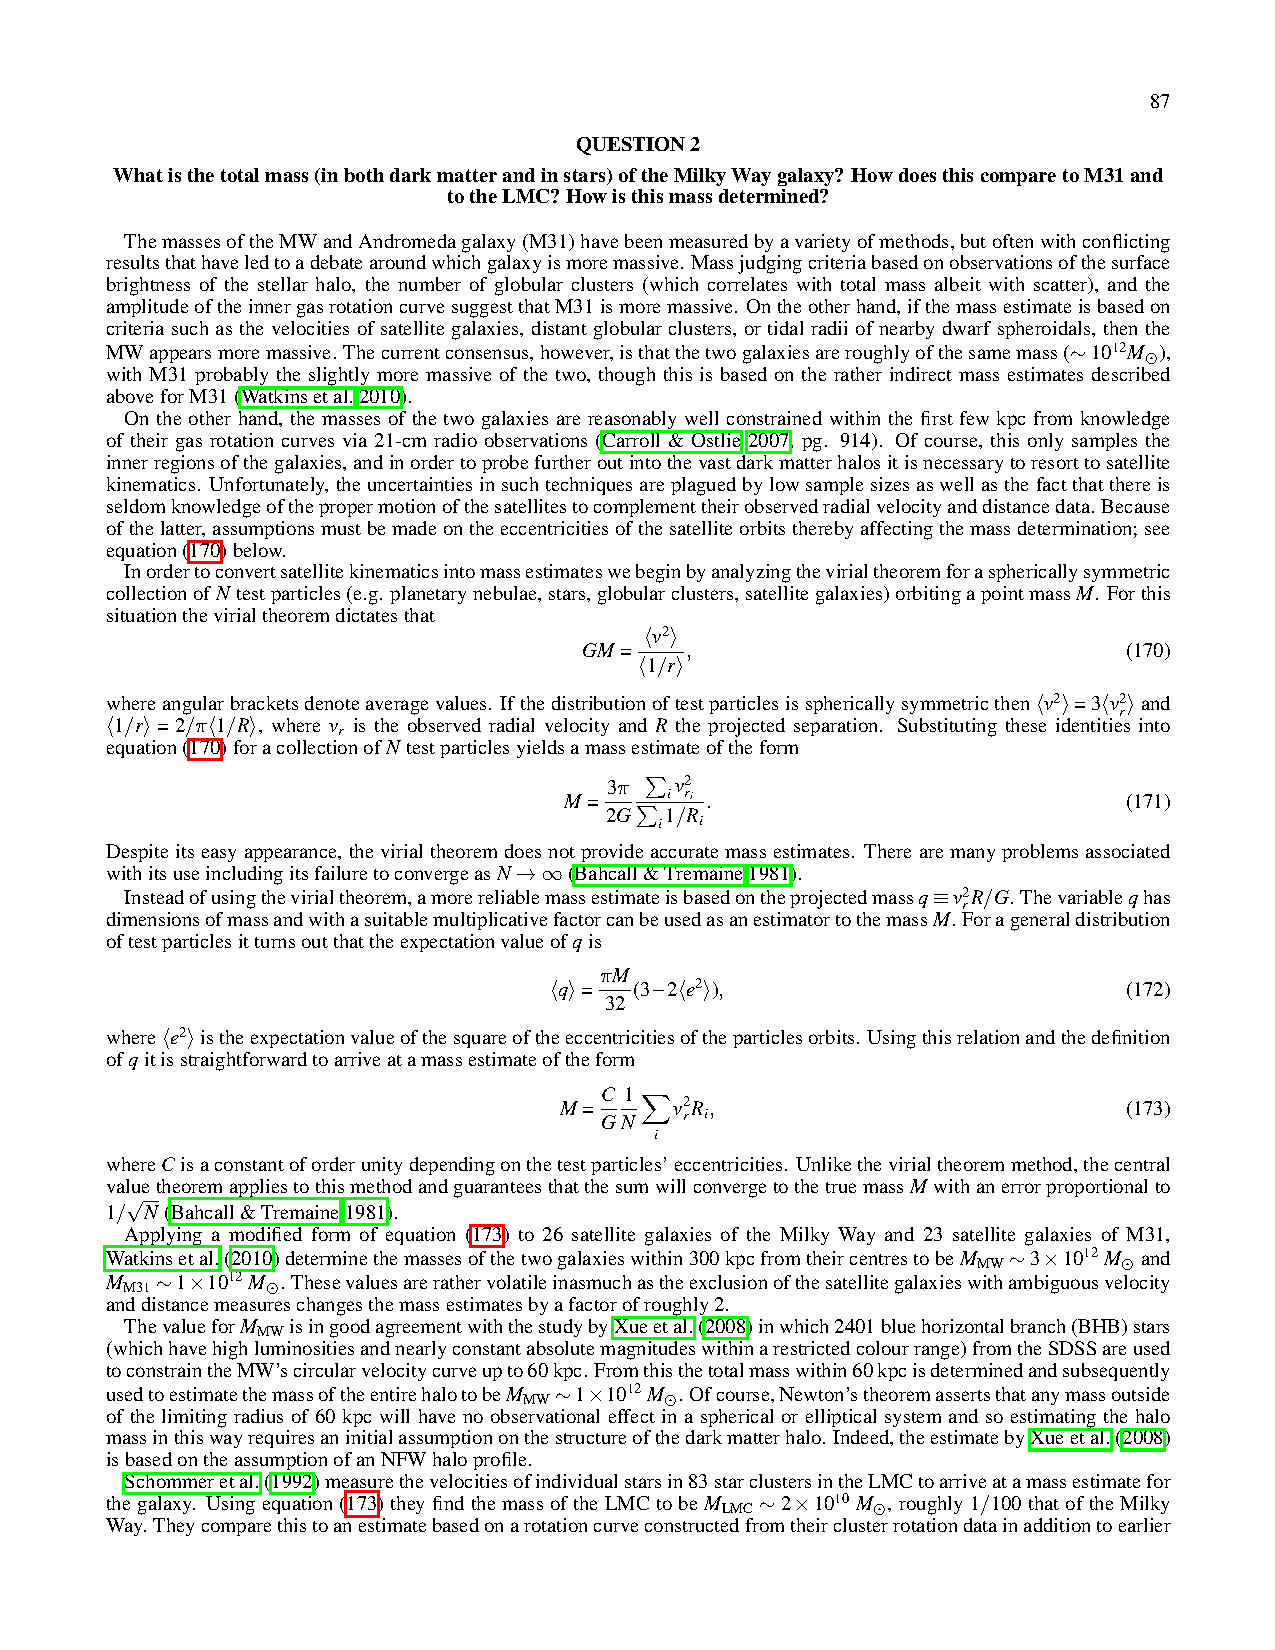
\includepdf[pagecommand=\subsection{Q1) Emberson ExtraGal Q2},scale=.93,offset=0 -14,pages=1]{galaxies/Emberson/Q1}\includepdf[pagecommand=\large{Q1) Emberson ExtraGal Q2},scale=.93,offset=0 -14,pages=2]{galaxies/Emberson/Q1}

	\includepdf[pagecommand=\subsection{Q1) Campbell ExtraGal Q2},scale=.93,offset=0 -14,pages=9]{galaxies/Campbell/extragalactic.pdf}\includepdf[pagecommand=\large{Q1) Campbell ExtraGal Q2},scale=.93,offset=0 -14,pages=10]{galaxies/Campbell/extragalactic.pdf}


% section q1_mass_of_the_milky_way (end)


% -----------------------------------------------------------------------------

\section{Q2) Nuclear Black Holes} % (fold)
\label{sec:q2_nuclear_black_holes}
\questiontext{What evidence is there that most galaxies contain nuclear black holes? How do those black holes interact with their host galaxies?}

    \subsection{Short Answer}
        \begin{itemize}
            \item stars: radial velocities (not PM) $\sigma \propto r^{-1/2}$
            \item gas: width of emission lines (doppler broadening) for radial velocity. Look for clumps of gas ? or do by annuli?
            \item masers: Doppler shifting of lase-light over time. emitted by water clouds. Masers are beamed (?).
            \item AGN
            \item EHT
        \end{itemize}{}
        
        Size and shape of BH gives mass and spin
        EHT did image in 1.3 mm, one of the shortest VLBI wavelengths.
        
        radius of influence of BH $\frac{GM}{R^2} \propto \sigma^2$
        from virial theorem $T=.5V^2 \sim 1.5 \sigma^2$, $U\sim .6 GM/R$, $2T=U$
        
        Mass-Luminosity relationship $M_b = 3e3 M_{bulge}$
        M-$\sigma$ relationship
    
    \includepdf[pagecommand=\subsection{Q2) Herman ExtraGal Q4},scale=.93,offset=0 -14,pages=4]{galaxies/Herman/2_Extragalactic.pdf}

    \includepdf[pagecommand=\subsection{Q2) Campbell ExtraGal Q4},scale=.93,offset=0 -14,pages=19]{galaxies/Campbell/extragalactic.pdf} \includepdf[pagecommand=\large{Q2) Campbell ExtraGal Q4},scale=.93,offset=0 -14,pages=20-22]{galaxies/Campbell/extragalactic.pdf}
        
% section q2_nuclear_black_holes (end)


% -----------------------------------------------------------------------------

\section{Q3) AGN} % (fold)
\label{sec:q3_agn}
\questiontext{What are AGN? Describe different observational classes of them and how they may relate to each other.}

% section q3_agn (end)
% External Answers
\includepdf[pagecommand=\subsection{Q3) Herman ExtraGal Q12},scale=.93,offset=0 -14,pages=12]{galaxies/Herman/2_Extragalactic}

\includepdf[pagecommand=\subsection{Q2) Campbell ExtraGal Q4},scale=.93,offset=0 -14,pages=44-46]{galaxies/Campbell/extragalactic.pdf} 
% -----------------------------------------------------------------------------

\section{Q4) Quasars} % (fold)
\label{sec:q4_quasars}
\questiontext{Draw a spectrum of a high-redshift quasar. What do quasar emission lines typically look like? Explain what we see in the spectrum at rest wavelengths bluer than 1216 Angstroms.}

% section q4_quasars (end)


% -----------------------------------------------------------------------------

\section{Q5) Methods of Galaxy Mass Determination} % (fold)
\label{sec:q5_methods_of_galaxy_mass_determination}
\questiontext{Describe three different methods used in the determination of the mass of a galaxy cluster.}

% section q5_methods_of_galaxy_mass_determination (end)


% -----------------------------------------------------------------------------

\section{Q6) SEDs of Single-Burst Galaxies} % (fold)
\label{sec:q6_seds_of_single_burst_galaxies}
\questiontext{Draw the spectral energy distribution (SED) of a galaxy formed by a single burst of star formation at the ages of 10 Myrs, 2 Gyrs, and 10 Gyr. Please highlight the change over time in the 4000 Angstrom break.}

% section q6_seds_of_single_burst_galaxies (end)


% -----------------------------------------------------------------------------

\section{Q7) Galactic Spiral Structure} % (fold)
\label{sec:q7_galactic_spiral_structure}
\questiontext{What is galactic spiral structure and why is it thought to occur?}

% section q7_galactic_spiral_structure (end)


% -----------------------------------------------------------------------------

\section{Q8) Stellar Initial Mass Funciton (IMF)} % (fold)
\label{sec:q8_stellar_initial_mass_funciton}
\questiontext{What is a stellar Initial Mass Function (IMF)? Explain how it is determined and how it is used.}

% section q8_stellar_initial_mass_funciton (end)


% -----------------------------------------------------------------------------

\section{Q9) Stellar Populations in the Galaxy} % (fold)
\label{sec:q9_stellar_populations_in_the_galaxy}
\questiontext{Characterize the stellar populations in the following regions: i) the Galactic bulge ii) the Galactic disk, outside of star clusters iii) open star clusters iv) globular clusters v) the Galactic halo}

% section q9_stellar_populations_in_the_galaxy (end)


% -----------------------------------------------------------------------------

\section{Q10) G-Dwarf Problem in the Solar Neighbourhood} % (fold)
\label{sec:q10_g_dwarf_problem_in_the_solar_neighbourhood}
\questiontext{What is the G-dwarf problem in the solar neighbourhood?}

% section q10_g_dwarf_problem_in_the_solar_neighbourhood (end)


% -----------------------------------------------------------------------------

\section{Q11) Stellar Orbits in Potential} % (fold)
\label{sec:q11_stellar_orbits_in_potential}
\questiontext{Describe the orbits of stars in a galactic disk and in galactic spheroid.}

% section q11_stellar_orbits_in_potential (end)


% -----------------------------------------------------------------------------

\section{Q12) Dynamical Relaxation} % (fold)
\label{sec:q12_dynamical_relaxation}
\questiontext{What is dynamical relaxation? Explain why this operates in star clusters but not
in an elliptical galaxy.}

% section q12_dynamical_relaxation (end)


% -----------------------------------------------------------------------------

\section{Q13) Dynamical Friction} % (fold)
\label{sec:q13_dynamical_friction}
\questiontext{What is dynamical friction? Explain how this operates in the merger of a small galaxy into a large one.}

% section q13_dynamical_friction (end)


% -----------------------------------------------------------------------------




% -----------------------------------------------------------------------------




% -----------------------------------------------------------------------------




% -----------------------------------------------------------------------------




% -----------------------------------------------------------------------------




% -----------------------------------------------------------------------------


%%%%%%%%%%%%%%%%%%%%%%%%%%%%%%%%%%%%%%%%%%%%%%%%%%%%%%%%%%%%%%%%%%%%%%%%%%%%%%%

\end{document}
